\documentclass[reqno,a4paper,12pt]{amsart}

\usepackage{amsmath,amssymb,amsthm,geometry,xcolor,soul,graphicx}
\usepackage{titlesec}
\usepackage{braket}
\usepackage{xeCJK}
\setCJKmainfont{Kai}
\geometry{left=0.7in, right=0.7in, top=1in, bottom=1in}


\renewcommand{\baselinestretch}{1.3}

\title{固体物理第一次作业}
\author{董建宇 ~~ 2019511017}

\begin{document}

\maketitle
\titleformat{\section}[hang]{\small}{\thesection}{0.8em}{}{}
\titleformat{\subsection}[hang]{\small}{\thesubsection}{0.8em}{}{}


\section{(2.2)}
\begin{enumerate}
	\item (德拜固体热熔假设): \\
	假设固体中存在$3N$个简正振动,且谐振子存在线性色散关系$\omega = v k$,其中$v$为波速,且频率存在截止频率$\omega_{cutoff}$,满足$3N = \int_0^{\omega_{cutoff}} 12\pi \left( \frac{L}{2\pi} \right)^3 \frac{\omega^2}{v^3}\,d\omega$;能级分立,一个特定频率$\omega_i$的谐振子平均能量为$\hbar\omega_i\left( \frac{1}{2} + \frac{1}{e^{\beta\hbar\omega_i} - 1} \right)$;边界条件满足Born-von Karmen Period Boundary Condition。 \\
	
	\item (计算德拜固体热熔): \\
	在三维固体中,平均能量为:
	\begin{equation*}
	\begin{aligned}
		\langle Q \rangle =& 3\sum_{k} \hbar\omega\left( \frac{1}{2} + \frac{1}{e^{\beta\hbar\omega} - 1} \right) \\
		=& 3\left( \frac{L}{2\pi} \right)^3 \int \,d\vec{k} \hbar\omega \left( \frac{1}{2} + \frac{1}{e^{\beta\hbar\omega} - 1} \right) \\
		=& \left( \frac{L}{2\pi} \right)^3 \frac{12\pi\hbar}{v^3} \int_{0}^{\omega_{cutoff}} \frac{\omega^3 \,d\omega}{e^{\beta\hbar\omega} - 1} + T ~ independent ~ constant.
	\end{aligned}
	\end{equation*}
	令$\omega_d = \omega_{cutoff}$,则热熔为:
	\begin{equation*}
	\begin{aligned}
		C = \frac{d\langle Q \rangle}{dT} = \left( \frac{L}{2\pi} \right)^3 \frac{12\pi\hbar^2}{v^3k_BT^2}\int_0^{\omega_d}\frac{\omega^4 e^{\beta\hbar\omega}}{(e^{\beta\hbar\omega}-1)^2}\,d\omega.
	\end{aligned}
	\end{equation*}
	令$x = \beta\hbar\omega$,则上式积分可写为:
	\[
		C = \left( \frac{L}{2\pi} \right)^3 \frac{12\pi k_B}{v^3(\beta\hbar)^3} \int_0^{\beta\hbar\omega_d} \frac{x^4e^x}{(e^x-1)^2}\,dx.
	\]
	令$k_BT_D = \hbar\omega_d$,其中$\omega_d^3 = \frac{6\pi^2Nv^3}{L^3}$。则热熔可以写为:
	\[
		C = 9Nk_B \frac{T^3}{T_D^3} \int_0^{\beta\hbar\omega_d} \frac{x^4e^x}{(e^x-1)^2}\,dx.
	\]
	对于低温极限,$\beta = \frac{1}{k_BT} \to +\infty$,则有:
	\[
		C = 9Nk_B \frac{T^3}{T_D^3}\int_0^{+\infty} \frac{x^4e^x}{(e^x-1)^2}\,dx = \frac{12\pi^4Nk_B}{5}\left(\frac{T}{T_D}\right)^3.
	\]
	对于高温极限,$\beta = \frac{1}{k_BT} \to 0$,则有:
	\[
		C = 9Nk_B \frac{T^3}{T_D^3} \int_0^{\beta\hbar\omega_d}x^2\,dx = 3Nk_B.
	\]
	
	\item
	由(2)可知,在低温极限下德拜温度与温度和热熔的关系为:
	\[
		T_D = T \sqrt[3]{\frac{12\pi^4k_BN_A}{5C}}.
	\]
	其中$N_A$为阿伏伽德罗常数。表格如下
	\begin{table}[h]
	\begin{tabular}{|l|l|l|l|l|l|l|l|}
	\hline
		T/K & 0.1 & 1.0 & 5 & 8 & 10 & 15 & 20 \\ \hline
		$C/(J K^{-1}mol^{-1})$ & $8.5\times 10^{-7}$ & $8.6\times 10^{-4}$ & 0.12 & 0.59 & 1.1 & 2.8 & 6.3 \\ \hline
		$T_D/K$ & 132.2 & 131.2 & 126.5 & 119.0 & 120.9 & 132.8 & 135.1 \\ \hline
	\end{tabular}
	\end{table} \\
	德拜固体热熔模型是在低温极限下近似得到热熔正比于温度的三次方,因此估计德拜温度约为
	\[
		T_D \approx 132K.
	\]
	同时从表中数据可知,在低温极限下,德拜温度近似相等,也就是说$T^3$是一个很好的近似。当温度上升时,计算出的德拜温度会出现较大波动,此时$T^3$近似误差会增加。
\end{enumerate}

\section{(2.3)}
\begin{enumerate}
	\item (二维德拜固体热熔假设):\\
	固体中$N$个原子存在$2N$个简正振动,且谐振子存在线性色散关系$\omega = v k$,且存在一个截止频率$\omega_{cutoff} = \omega_d$,满足$2N = \int_0^{\omega_{d}}\frac{L^2\omega}{\pi v^2}\,d\omega$;能级分立,对于给定温度,频率为$\omega_i$的振子能量为$E_i = \hbar\omega_i \left( \frac{1}{2} + \frac{1}{e^{\beta\hbar\omega_i} -  1} \right)$;边界条件满足Born-von Karmen Period Boundary Condition。
	
	\item (计算热熔): \\
	在二维固体中,平均能量为:
	\begin{equation*}
	\begin{aligned}
		\langle Q \rangle =& 2\sum_k \hbar\omega \left( \frac{1}{2} + \frac{1}{e^{\beta\hbar\omega_i} -  1} \right) \\
		=& 2\frac{L^2}{4\pi^2} \int_0^{\omega_d} 2\pi \frac{\omega}{v^2}\hbar\omega \left( \frac{1}{2} + \frac{1}{e^{\beta\hbar\omega_i} -  1} \right) \,d\omega \\
		=& \frac{\hbar L^2}{\pi v^2} \int_0^{\omega_d} \frac{\omega^2}{e^{\beta\hbar\omega} - 1}\,d\omega + T ~ independent ~ constant.
	\end{aligned}
	\end{equation*}
	则热熔为:
	\[
		C = \frac{d\langle Q \rangle}{dT} = \frac{\hbar^2L^2k_B\beta^2}{\pi v^2} \int_0^{\omega_d} \frac{\omega^3e^{\beta\hbar\omega}}{(e^{\beta\hbar\omega}-1)^2}\,d\omega.
	\]
	令$x = \beta\hbar\omega$,则积分可以写为:
	\[
		C = \frac{L^2k_B}{\pi v^2(\beta\hbar)^2} \int_0^{\beta\hbar\omega_d} \frac{x^3e^x}{(e^x - 1)^2}\,dx.
	\]
	
	\item (高温极限): \\
	对于高温极限,$\beta = \frac{1}{k_BT}\to 0$,则有:
	\[
		C = \frac{L^2k_B}{\pi v^2(\beta\hbar)^2} \int_0^{\beta\hbar\omega_d} x\,dx = \frac{L^2k_B\omega_d^2}{2\pi v^2}.
	\]
	由截止频率定义可知:
	\[
		2N = \int_0^{\omega_d} \frac{L^2\omega}{\pi v^2}\,d\omega = \frac{L^2\omega_d^2}{2\pi v^2}.
	\]
	则有:
	\[
		\omega_d^2 = \frac{4N\pi v^2}{L^2}.
	\]
	则在高温极限下,热熔为:
	\[
		C = 2Nk_B.
	\]
	
	\item (低温极限): \\
	对于低温极限,$\beta = \frac{1}{k_BT} \to +\infty$,则有:
	\[
		C = \frac{L^2k_B}{\pi v^2(\beta \hbar)^2} \int_0^{+\infty} \frac{x^3e^x}{(e^x - 1)^2}\,dx = KT^2.
	\]
	即$n = 2$,其中
	\[
		K = \frac{L^2k_B^3}{\pi v^2\hbar^2} \int_0^{+\infty} \frac{x^3e^x}{(e^x - 1)^2}\,dx.
	\]
\end{enumerate}

\section{(2.4)}
\begin{enumerate}
	\item (最高德拜温度): \\
	对于三维固体,有
	\[
		\omega_d^3 = \frac{6\pi^2 Nv^3}{L^3}, ~ k_BT_D = \hbar\omega_d.
	\]
	则要使德拜温度最高,需要使德拜截止频率最大,即使原子振动频率最大,或者使固体中声速最大。因此杨氏模量越大、密度越小的固体,有可能具有更高的德拜温度。结合课本信息可以猜测金刚石(diamond)具有最高的德拜温度。
	
	\item (最低德拜温度): \\
	要使德拜温度最低,需要使德拜截止频率最小,因此杨氏模量越小(越软)、密度越大的固体,有可能会具有更低的德拜温度。因此猜测汞(水银)具有最低的德拜温度,因为水银在常温下为液体,杨氏模量较小,同时汞在常温下密度为$13.6g/cm^3$较大。
\end{enumerate}

\section{(2.5)}
\begin{enumerate}
	\item (估计金刚石德拜温度): \\
	从图中可读出,当温度为$T = 59K$时,热熔约为
	\[
		C_p = 0.038(J\cdot mol^{-1}\cdot K^{-1}).
	\]
	由理论推导可知,热熔与温度的三次方成正比,则对于三维金刚石斜率为:
	\[
		\frac{12\pi^4N_Ak_B}{5T_D^3} = \frac{C_p}{T^3}
	\]
	则金刚石德拜温度估计值为:
	\[
		T_D = 2189.8K.
	\]
	
	\item (与表中数据不匹配原因): \\
	德拜固体热熔模型是在低温极限下近似得到热熔正比于温度的三次方,而图中$59K$的温度可能使得近似误差增大,从而导致了金刚石的德拜温度估计值高。同时,表2.2中数据是在标准温度和压强下测量得到,而材料的实际德拜温度可能受环境温度等因素的影响,从而导致估计值偏离标准温度和压强下的测量值。
\end{enumerate}

\section{(补充习题)}
\begin{enumerate}
	\item (绘图): \\
	单位划算为:
	\[
		1Cal = 4.1859J, ~ 1g~atom = 1 mol.
	\]
	即有:
	\[
		1Cal/(g~atom)K = 4.1859J/mol~K.
	\]
	利用Matlab绘图如下: \\
	Ge的热熔随温度变化散点图为:\\
	\begin{center}
		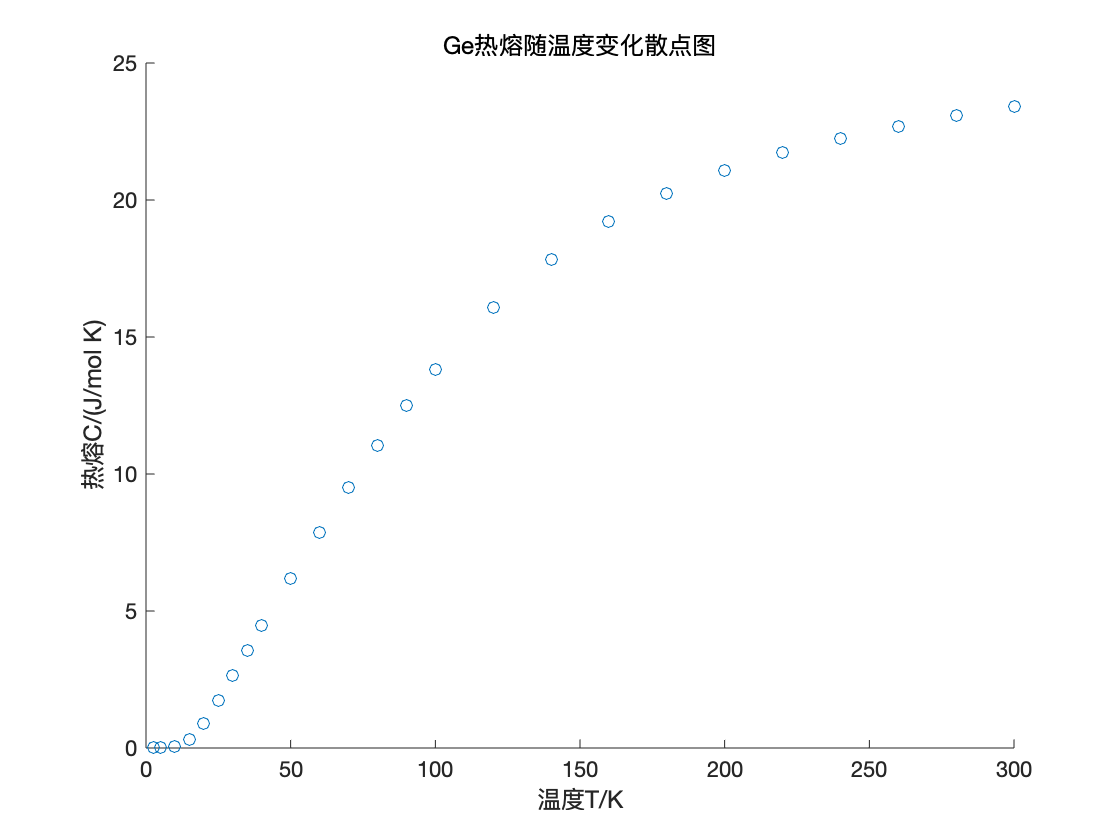
\includegraphics[scale = 0.3]{Ge_C_T.png}
	\end{center}
	在$T = 300K$时,Ge热熔与Dulong Petit极限$3R$比值为:
	\[
		\eta_{Ge} = \frac{23.4}{3\times 8.31} = 93.0\%.
	\]
	Si的热熔随温度变化散点图为:\\
	\begin{center}
		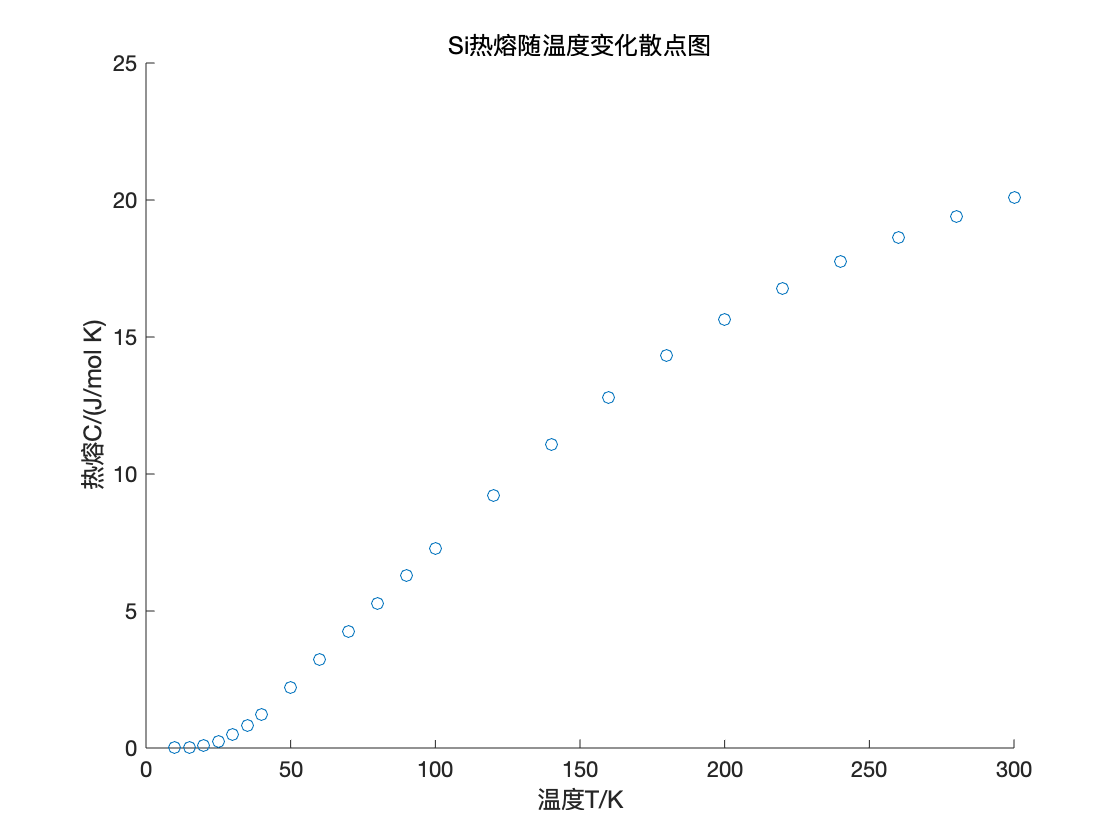
\includegraphics[scale = 0.3]{Si_C_T.png}
	\end{center}
	在$T = 300K$时,Si热熔与Dulong Petit极限$3R$比值为:
	\[
		\eta_{Si} = \frac{20.08}{3\times 8.31} = 80.5\%.
	\]
	$\eta_{Ge} > \eta_{Si}$,也就是说在$T = 300K$条件下,Ge的热熔比Si的热熔更接近于Dulong Petit极限,也就意味着Ge的德拜温度低于Si的德拜温度。
	
	\item (分析Ge的热熔在10K及以下是否服从$T^3$关系): \\
	利用Matlab绘制10K及以下的Ge的热熔随温度三次方的散点图并用直线拟合如下:
	\begin{center}
		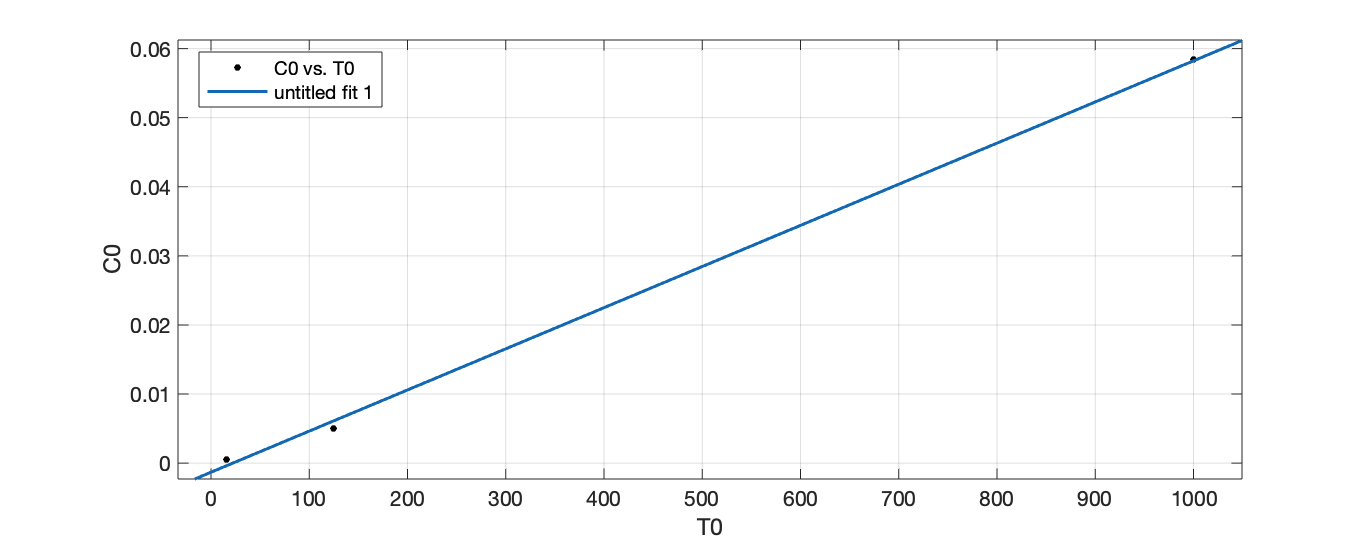
\includegraphics[scale = 0.3]{Ge_C_T_less10K.png}
	\end{center}
	\begin{center}
		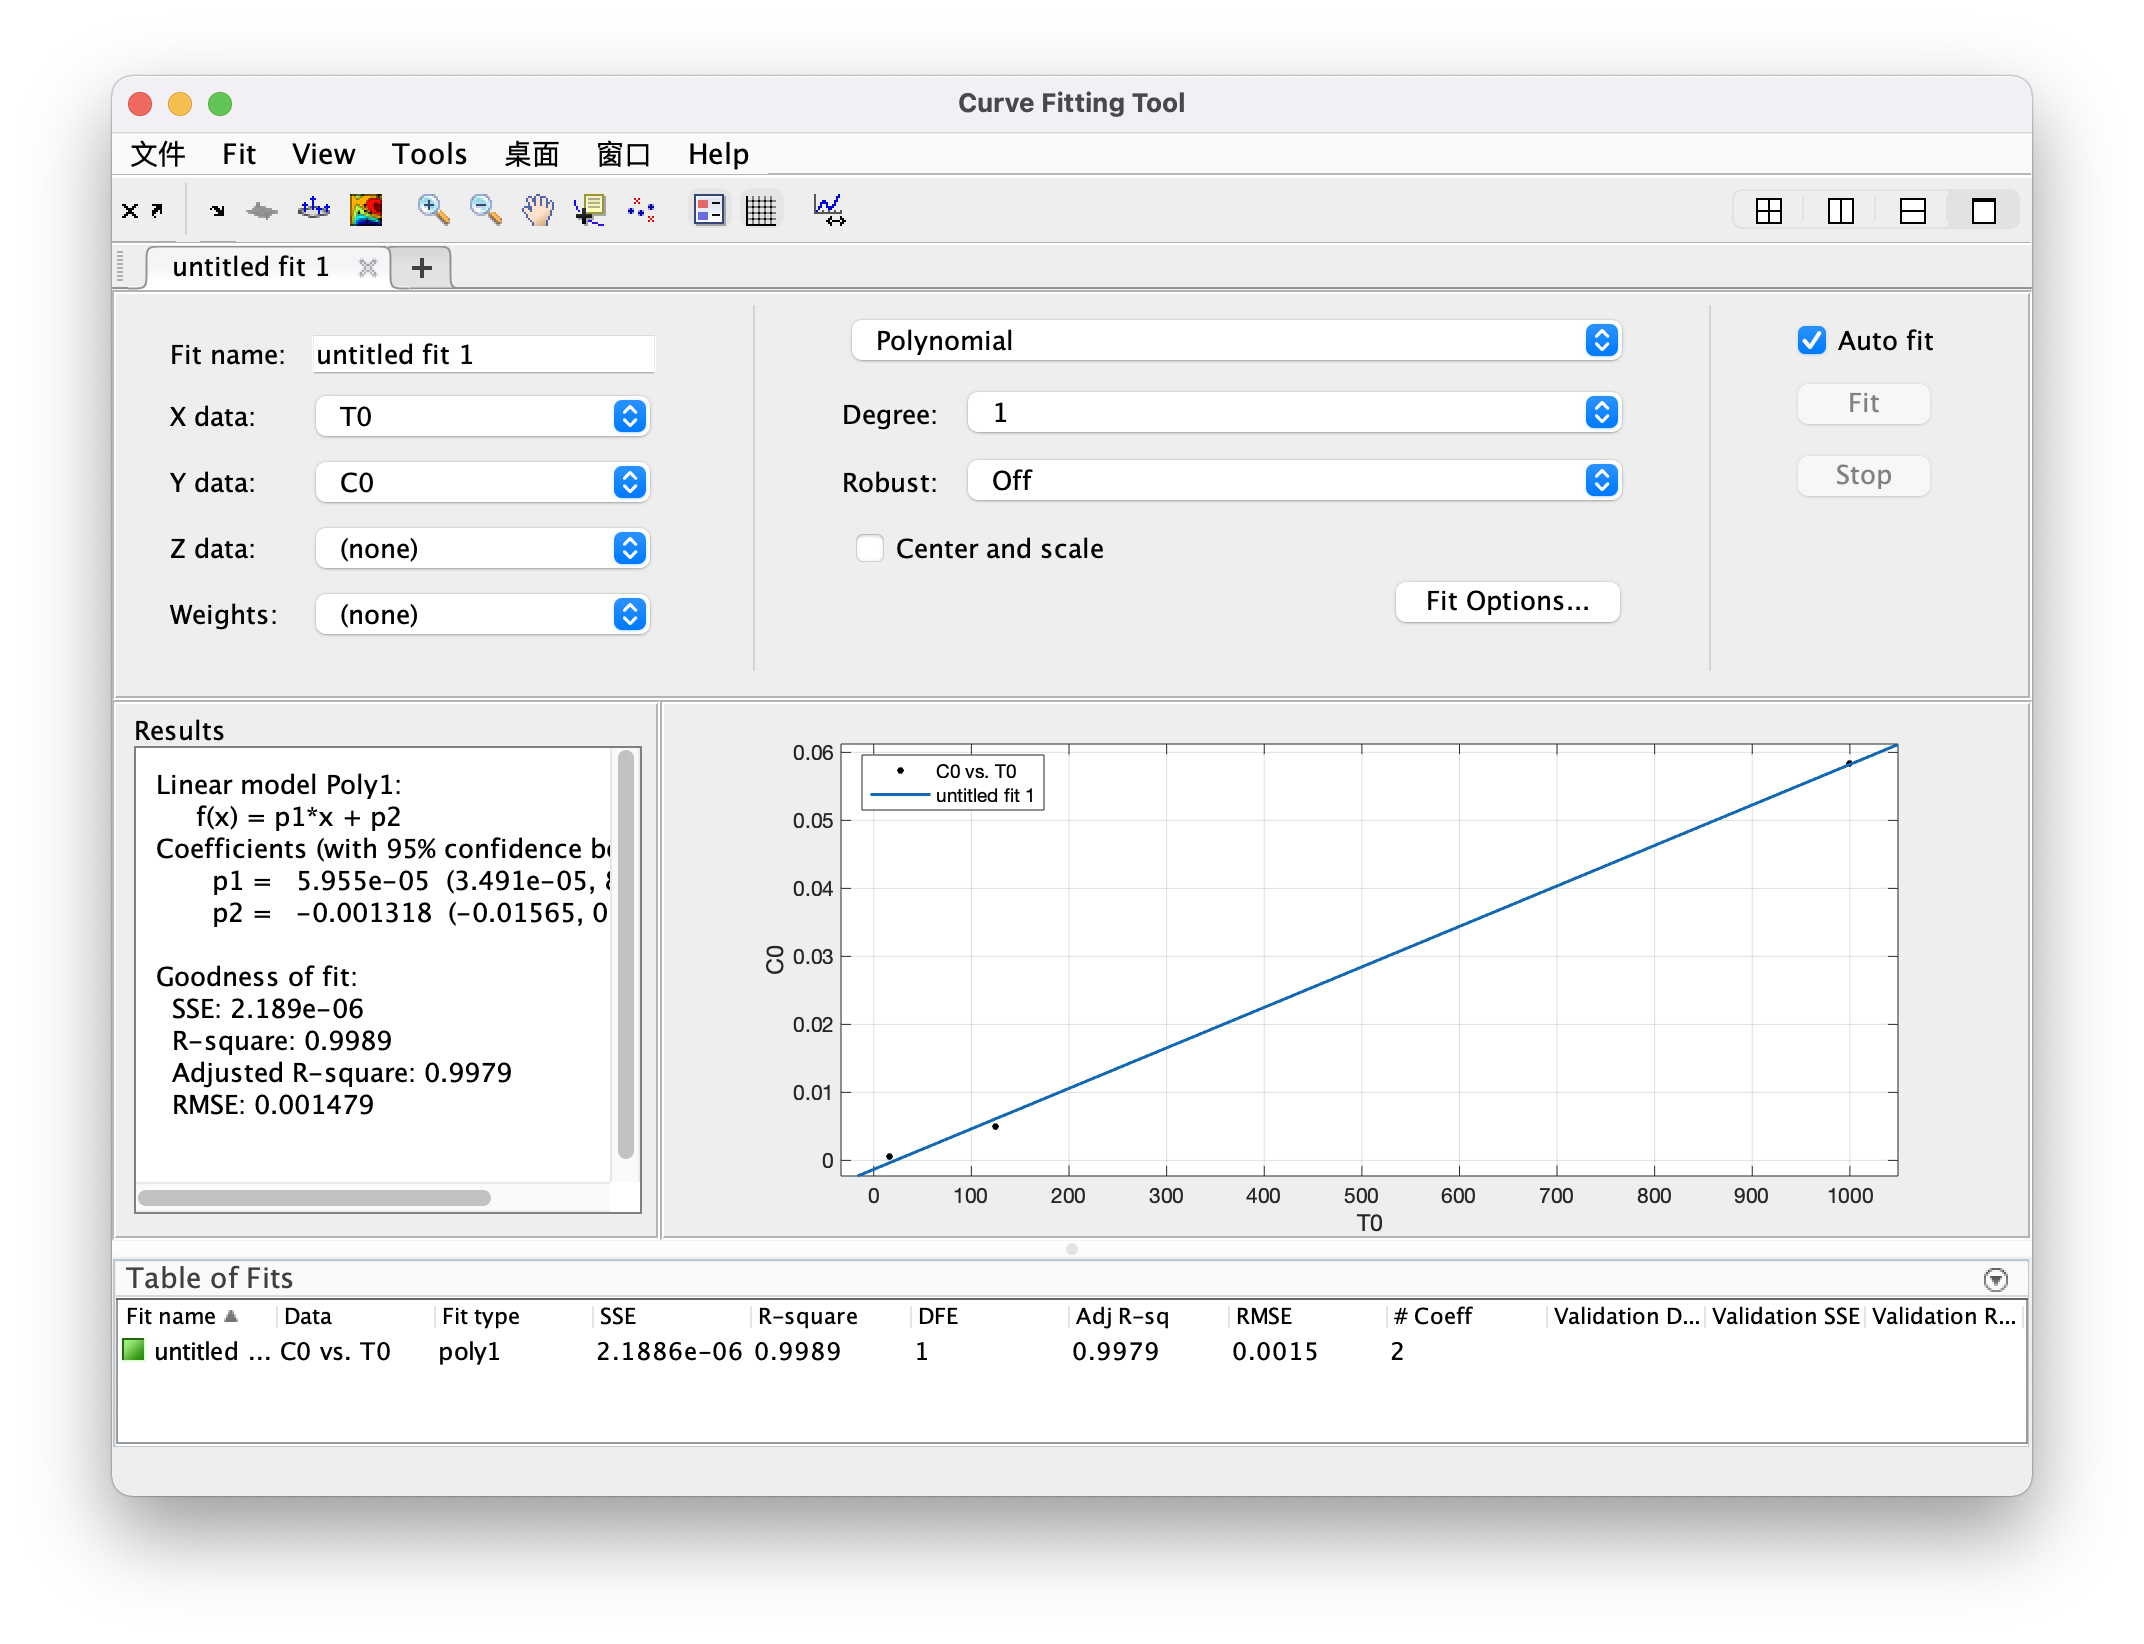
\includegraphics[scale = 0.3]{Ge_C_T_less10Kdata.png}
	\end{center}
	拟合直线相关系数为$R^2 = 0.9989 > 0.99$,即可以认为Ge的热熔在10K及以下的数据服从$T^3$关系。
	
	\item (估计Ge的德拜温度): \\
	由上述拟合直线的斜率大小为$m = 5.96\times 10^{-5}$,可以计算Ge的德拜温度估计值为:
	\[
		T_{Ge} = \sqrt[3]{\frac{12\pi^4k_BN_A}{5m}} \approx 319.4K.
	\]
	
	\item (估计Si的德拜温度): \\
	由Si在10K的热熔,计算Si的德拜温度估计值为:
	\[
		T_{Si} = T\sqrt[3]{\frac{12\pi^4k_BN_A}{5C}} \approx 630.8K.
	\]
\end{enumerate}


\end{document}